\documentclass[12pt]{article}

% ----------------------------------------------------------------------
% Define external packages, language, margins, fonts, new commands 
% and colors
% ----------------------------------------------------------------------
\usepackage[utf8]{inputenc} % Codification
\usepackage[english]{babel} % Writing idiom

\usepackage{graphicx}
\usepackage[export]{adjustbox} % Align images
\usepackage{amsmath} % Extra commands for math mode
\usepackage{amssymb} % Mathematical symbols
\usepackage{anysize} % Personalize margins
    \marginsize{2cm}{2cm}{2cm}{2cm} % {left}{right}{above}{below}
\usepackage{appendix} % Appendices
\usepackage{cancel} % Expression cancellation
\usepackage{caption} % Captions
    \captionsetup{labelfont={bf}}
\usepackage{cite} % Citations, like [1 - 3]
\usepackage{color} % Text coloring
\usepackage{fancyhdr} % Head note and footnote
    \pagestyle{fancy}
    \fancyhf{}
    \fancyhead[L]{\footnotesize IST} % Left of Head note
    \fancyhead[R]{\footnotesize ULisboa} % Right of Head note
    \fancyfoot[L]{\footnotesize SAAR} % Left of Footnote
    \fancyfoot[C]{\thepage} % Center of Footnote
    \fancyfoot[R]{\footnotesize METI} % Right of Footnote
    \renewcommand{\footrulewidth}{0.4pt} % Footnote rule
\usepackage{float} % Utilization of [H] in figures
\usepackage{graphicx} % Figures in LaTeX
\usepackage[colorlinks = true, plainpages = true, linkcolor = istblue, urlcolor = istblue, citecolor = istblue, anchorcolor = istblue]{hyperref}
\usepackage{indentfirst} % First paragraph
\usepackage[super]{nth} % Superscripts
\usepackage{siunitx} % SI units
\usepackage{subcaption} % Subfigures
\usepackage{titlesec} % Font
    \titleformat{\section}{\Large\bfseries}{\thesection}{1em}{}
    \titleformat{\subsection}{\large\bfseries}{\thesubsection}{1em}{}
    \titleformat{\subsubsection}{\normalsize\bfseries}{\thesubsubsection}{1em}{}
    \fancyfoot[C]{\thepage}

% Random text (not needed)
\usepackage{lipsum}
\usepackage{duckuments}

% New and re-newcommands
\newcommand{\sen}{\operatorname{\sen}} % Sine function definition
\newcommand{\HRule}{\rule{\linewidth}{0.5mm}} % Specific rule definition
\renewcommand{\appendixpagename}{\LARGE Appendices}

% Colors
\definecolor{istblue}{RGB}{3, 171, 230}
\definecolor{dkgreen}{rgb}{0,0.6,0}
\definecolor{gray}{rgb}{0.5,0.5,0.5}

%%%%%%%%%%%%%%%%%%%%%%%%%%%%%%%%%%%%%%%%%%%%%%%%%%%%%%%%%%%%%%%%%%%%%%%%
%                                 Document                             %
%%%%%%%%%%%%%%%%%%%%%%%%%%%%%%%%%%%%%%%%%%%%%%%%%%%%%%%%%%%%%%%%%%%%%%%%
\begin{document}

% ----------------------------------------------------------------------
% Cover
% ----------------------------------------------------------------------
\begin{center}
    \begin{figure}
        \vspace{-1.0cm}
        
\includegraphics[scale = 0.25, left]{../Images/IST_A.png} % IST logo
    \end{figure}
    \mbox{}\\[2.0cm]
    \textsc{\Huge Advanced Network Security and Architectures}\\[2.5cm]
    \textsc{\LARGE METI}\\[2.0cm]
    \HRule\\[0.4cm]
    {\large \bf {Report Module 1} [\texttt{EN}]}\\[0.2cm]
    \HRule\\[1.5cm]
\end{center}

\begin{flushleft}
    \textbf{Authors:}
\end{flushleft}

\begin{center}
    \begin{minipage}{0.5\textwidth}
        \begin{flushleft}
            José Oliveira (103771)\\
            Afonso Mendes (116024)\\
            Tiago Videira (116069)
        \end{flushleft}
    \end{minipage}%
    \begin{minipage}{0.5\textwidth}
        \begin{flushright}
            \href{mailto:jose.novais.oliveira@tecnico.ulisboa.pt}{\texttt{jose.novais.oliveira@tecnico.ulisboa.pt}}\\
            \href{mailto:afonsofmendes@tecnico.ulisboa.pt}{\texttt{afonsofmendes@tecnico.ulisboa.pt}}\\
            \href{mailto:tiago.g.videira@tecnico.ulisboa.pt}{\texttt{tiago.g.videira@tecnico.ulisboa.pt}}
        \end{flushright}
    \end{minipage}
\end{center}
    
\begin{flushleft}
    \large $\boxed{\text{\bf Group 3 }}$\\[4.0cm]
\end{flushleft}
    
\begin{center}
    \large \bf 2025/2026 -- \nth{2} Semester, P4
\end{center}

\thispagestyle{empty}

\setcounter{page}{0}

\newpage

% ----------------------------------------------------------------------
% Contents
% ----------------------------------------------------------------------
\tableofcontents 

\newpage

% ----------------------------------------------------------------------
% Body
% ----------------------------------------------------------------------

\section{Introduction}

FAZER APENAS NO FIM DOS 3 LABS

\newpage

\section {Network attacks and countermeasures}

\subsection{Objective}

The main objective of this laboratory work is to study and experimentally evaluate a set of common network attacks and their corresponding countermeasures in a controlled environment using GNS3.

In particular, the following attacks are addressed:

\begin{itemize}
    \item \textbf{MAC table overflow:} to understand how a switch can be forced to behave as a hub by saturating its MAC address table, and to evaluate mitigation mechanisms such as port security.
    
    \item \textbf{DHCP spoofing:} to demonstrate how a rogue DHCP server can provide malicious network configurations to clients, and to analyze the effectiveness of DHCP snooping as a countermeasure.
    
    \item \textbf{ARP poisoning (Man-in-the-Middle):} to perform a MitM attack by manipulating ARP tables, and to study the use of Dynamic ARP Inspection (DAI) for protection.
    
    \item \textbf{DNS spoofing:} to analyze how a victim can be redirected to a fake web server through DNS manipulation combined with ARP poisoning.
    
    \item \textbf{RIP poisoning:} to investigate how routing tables can be corrupted using forged RIP messages, leading to traffic redirection, and to explore authentication-based defenses.
\end{itemize}

Additionally, this work aims to:

\begin{itemize}
    \item Analyze network behavior through packet captures using Wireshark;
    \item Interpret device-level information using Cisco IOS commands;
    \item Evaluate the practical feasibility and limitations of each attack;
    \item Compare experimental results with theoretical expectations.
\end{itemize}

\newpage

\subsection{MAC Table Overflow}

\subsubsection{Attack and Countermeasure}  
The MAC table overflow attack was performed using the \texttt{camov.py} script, generating a large number of frames with different spoofed MAC addresses.  

As observed in Wireshark (Figure~\ref{fig:mac_overflow}), a high volume of traffic with varying source addresses was captured, indicating the flooding behavior of the attack.

The switch behavior was analyzed using \texttt{show mac address-table}.  

To mitigate the attack, port security was configured, limiting the number of MAC addresses per port and preventing the insertion of multiple spoofed entries.

\begin{figure}[h]
    \centering
    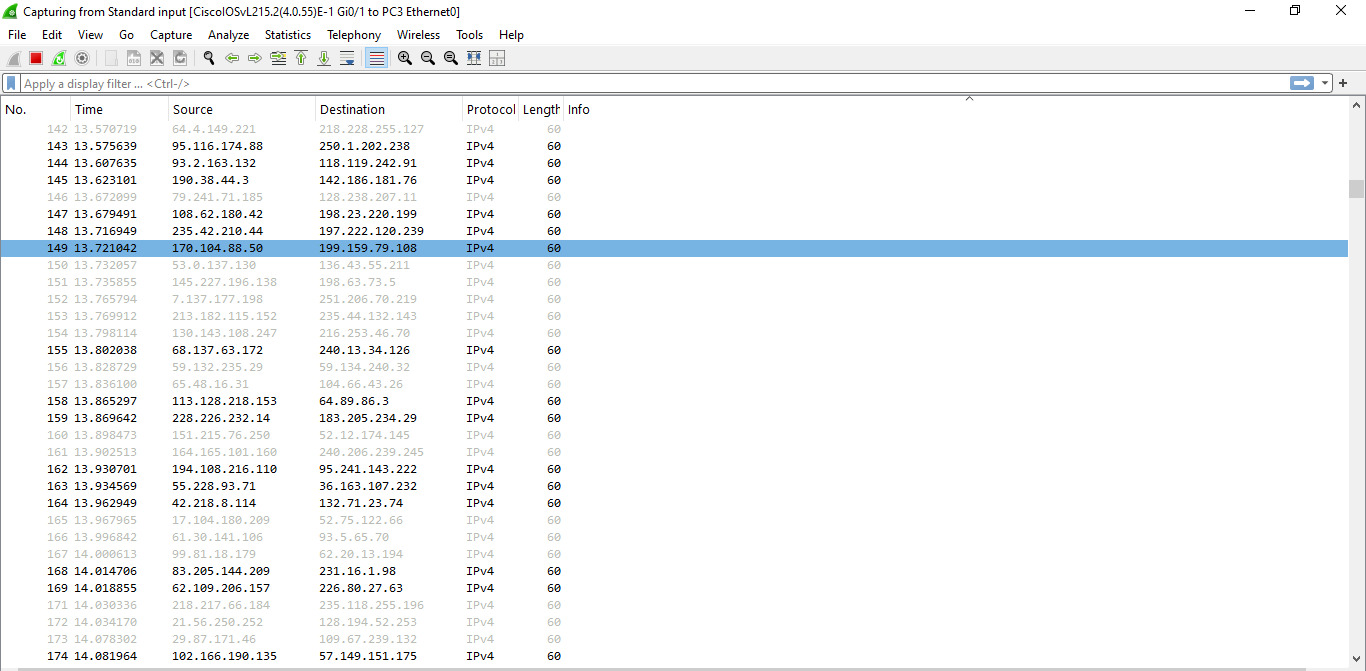
\includegraphics[width=1\linewidth]{../Images/wireshark1.jpeg}
    \caption{Wireshark capture during MAC table overflow attack}
    \label{fig:mac_overflow}
\end{figure}

\subsubsection{Switch Comparison}  

Cisco Catalyst 2960 supports port security, allowing the configuration of a maximum number of MAC addresses per port and defining actions when violations occur (e.g., restrict or shutdown). This makes it possible to prevent MAC table overflow attacks.

Link: \url{www.cisco.com/c/en/us/products/switches/catalyst-2960-series-switches/index.html}

\vspace{0.3cm}

In contrast, the TP-Link TL-SF1005D is an unmanaged switch that does not support port security or any traffic control mechanisms, as it lacks a configuration interface. Therefore, it cannot prevent MAC flooding attacks.

Link: \url{www.tp-link.com/en/home-networking/soho-switch/tl-sf1005d/}

\subsubsection{Feasibility}  
The objective of this attack is to flood the switch MAC address table, forcing the switch to behave like a hub. In that state, frames may be forwarded to all ports, allowing the attacker to listen to conversations between other hosts.

However, in practice, the attack may be difficult to execute successfully on modern switches because their MAC address tables are large. Additionally, the high amount of generated traffic can cause network instability or a denial-of-service condition, instead of allowing the attacker to reliably capture useful traffic.

Therefore, although the attack is theoretically possible, its practical feasibility is limited and depends on the switch capacity, configuration, and security features.

\subsection{DHCP spoofing}

\subsubsection{Attack and Countermeasure}  
The DHCP spoofing attack was performed by introducing a rogue DHCP server that responds to DHCP Discover messages with malicious configuration parameters.

As observed in Wireshark (Figure~\ref{fig:dhcp_attack}), multiple DHCP Offer messages were received for the same transaction ID, indicating a race condition between the legitimate and the rogue DHCP servers. The victim accepts the first Offer received, which may result in a malicious gateway configuration provided by the attacker.

\begin{figure}[h]
    \centering
    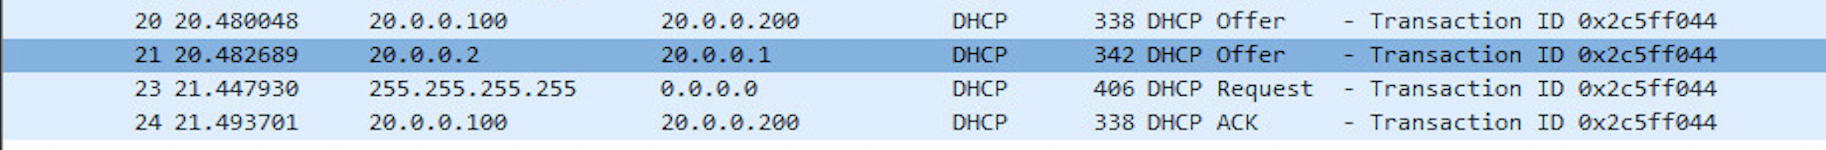
\includegraphics[width=1\linewidth]{../Images/wireshark2.png}
    \caption{Wireshark capture showing multiple DHCP Offer messages (attack)}
    \label{fig:dhcp_attack}
\end{figure}

After enabling DHCP snooping and configuring the port connected to the legitimate DHCP server as trusted, only one DHCP Offer was observed (Figure~\ref{fig:dhcp_snooping}). The rogue DHCP responses were blocked by the switch, and the client received a valid configuration. This confirms that DHCP snooping effectively mitigates the attack.

\begin{figure}[h]
    \centering
    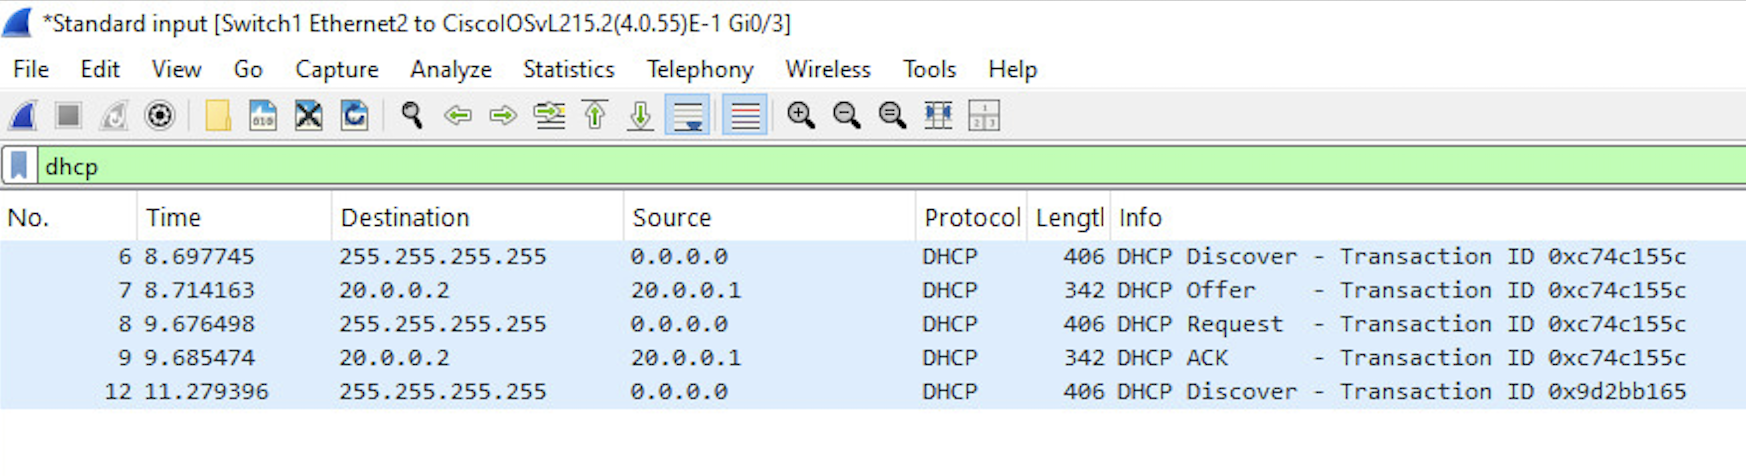
\includegraphics[width=1\linewidth]{../Images/wireshark3.png}
    \caption{Wireshark capture with DHCP snooping enabled (only legitimate Offer)}
    \label{fig:dhcp_snooping}
\end{figure}



\subsubsection{AI Prediction}  
The AI predicted that the victim closer to the attacker would be more likely to be compromised, since the rogue DHCP Offer would arrive first. This prediction matched the experimental results, where the victim receiving the first Offer obtained the malicious configuration.

\subsubsection{Switch Comparison}  
Cisco Catalyst 2960 supports DHCP snooping, allowing ports to be classified as trusted or untrusted and blocking DHCP server messages from untrusted ports.

Link: \url{www.cisco.com/c/en/us/products/switches/catalyst-2960-series-switches/index.html}

\vspace{0.3cm}

The TP-Link TL-SF1005D does not support DHCP snooping, as it is an unmanaged switch without configuration capabilities or security features.

Link: \url{www.tp-link.com/en/home-networking/soho-switch/tl-sf1005d/}

\subsubsection{Feasibility}  
The attack is feasible in networks without DHCP snooping, especially when the attacker is closer to the victim than the legitimate DHCP server. However, due to the race condition, success is not guaranteed. When DHCP snooping is enabled, the attack becomes ineffective.

\subsection{ARP poisoning (MitM)}

\subsection{DNS spoofing}

\subsection{RIP poisoning}



%% DAQUI PARA BAIXO LAB 2 E 3

\newpage

\section {Firewalls}

\newpage

\section {AAA}

\end{document}